\chapter{\IfLanguageName{dutch}{PoC}{PoC}}%
\label{ch:PoC}

\section{Inleiding}
Deze documentatie biedt een uitgebreid overzicht van een Proof of Concept (PoC) script dat is ontwikkeld voor het lokaal uitvoeren van een machine learning (ML) pipeline. Het script maakt gebruik van het Prefect-framework voor het orchestreren van de pipeline-taken en MLflow voor het bijhouden van experimenten en logging.
\section{Scenario}
In het onderdeel ``Machine Learning Operations'' van de opleiding kregen studenten een labo waarin ze een Machine Learning pipline moesten opzetten met behulp van Azure. De student diende een Python-script te openen in een Python-omgeving en dit script vervolgens te verbinden met de endpoint van de Azure-servers.
Hierdoor kon de Machine Learning pipeline worden uitgevoerd op de Azure-server. Het script betrof een classificatiemodel om appels van sinaasappels te onderscheiden, bestaande uit drie delen: preprocessing, training en evaluatie. De preprocessing-functie downloadde alle bestanden en paste ze aan naar een uniform formaat. Het trainingsgedeelte trainde het model, dat bestond uit verschillende Keras-lagen. Uiteindelijk werd het model geëvalueerd om de prestaties ervan te meten.
Voor dit Proof of Concept word het zelfde script gebruikt zoals in de labo van ``Machine Learning Operations''

\section{Probleemstelling}
Om gebruik te kunnen maken van de Azure-servers, hebben gebruikers credits nodig. Tijdens het eerder genoemde lab waren er studenten die voor aanvang of tijdens het lab geen credits meer hadden. Dit leidde ertoe dat deze studenten hun resultaten niet konden presenteren of zelfs niet konden beginnen aan het lab.
Daarom wordt in dit onderzoeksvoorstel gekeken naar het opzetten van een lokale installatie van een Machine Learning pipeline.
\section{Verwacht resultaat}
Het verwachtte resultaat is een framework dat een Machine Learning pipline lokaal kan uitvoeren en dat het framework voldoet aan alle criteria van de risicoanalyse.
\section{Uitvoering}
De uitvoering van deze Proof of Concept (PoC) zal worden uitgevoerd met behulp van het Prefect-framework samen met MLFlow. Prefect voldoet aan alle criteria van de risicoanalyse en heeft een niet al te steile leercurve, waardoor het een geschikte keuze is voor een labo binnen het opleidingsonderdeel ``Machine Learning Operations''.

Prefect biedt verschillende voordelen ten opzichte van andere frameworks. Ten eerste maakt het eenvoudig plannen van de pipeline mogelijk, zodat deze op een specifiek tijdstip kan worden uitgevoerd. Bovendien is Prefect een Python-bibliotheek, waardoor de enige vereiste kennis Python is, wat mag worden verwacht van de studenten. Daarnaast is het mogelijk om zelf een Prefect-server te starten, waardoor alles lokaal kan worden uitgevoerd, wat overeenkomt met het doel van deze proof of concept.

MLFlow zal ook worden gebruikt in deze Proof of Concept. Deze bibliotheek zal zorgen voor het bijhouden van metingen tijdens het machine learning proces. Dit omvat onder andere metingen zoals de nauwkeurigheid van het model, het verlies van het model, en het zal ook alle systeemeigenschappen bijhouden.

Prefect werkt met behulp van ``decorators'', die Prefect in staat stellen om Python-functies te herkennen en uit te voeren als een pipeline. De twee decorators die Prefect gebruikt zijn @task en @flow.

De @task decorator markeert een functie als een taak, waardoor meerdere taken kunnen worden samengevoegd in een stroom (flow) en in een specifieke volgorde kunnen worden uitgevoerd. Een voorbeeld van een taak in Prefect wordt hieronder gegeven:
\begin{minted}[frame=lines,breaklines, linenos]{python}
    @task
    def my_task():
        print("Hallo")
\end{minted}

In dit voorbeeld zal de taak ``Hallo'' uitvoeren en de naam van de functie dient ook als de naam van de taak.

De @flow decorator combineert alle taken en voert ze vervolgens uit. Een voorbeeld van een flow in Prefect wordt hieronder gegeven:
\begin{minted}[frame=lines,breaklines, linenos]{python}
    @flow(name="Test Flow")
    def main():
        my_task()
\end{minted}
In dit voorbeeld zal de flow de taak uitvoeren die eerder is gedefinieerd in een taak. Deze keer wordt een naam aan de flow gegeven, hoewel dit niet strikt noodzakelijk is, kan het helpen om de code overzichtelijker te maken. Er is geen maximumaantal taken dat aan een flow kan worden toegevoegd. Let op dat een taak niet zelfstandig kan worden uitgevoerd deze moet altijd binnen een flow worden geplaatst om te worden uitgevoerd.

De task en flows zijn de core van Prefect. Om te beginnen aan het PoC moet eerst alle nodige Python-biblitheken worden geinstalleer.
De biblitheken die werden gebruikt voor deze PoC zijn:
\begin{itemize}
    \item keras (versie 2.15.0)
    \item mlflow (versie 2.11.3)
    \item Requests (versie 2.31.0)
    \item tensorflow (versie 2.15.0)
\end{itemize}

% deze kunnen als volgt worden geinstalleerd: 

% \begin{minted}{text}
%     pip install keras==2.15.0 mlflow==2.11.3 requests==2.31.0 tensorflow==2.15.0 tensorflow_macos==2.15.0
% \end{minted}

% Dit PoC is gebaseerd op de notebook van labo 3 in het opleidingsonderdeel ``Machine Learning Operations''
% %github?

% % \begin{figure}[h]
% %     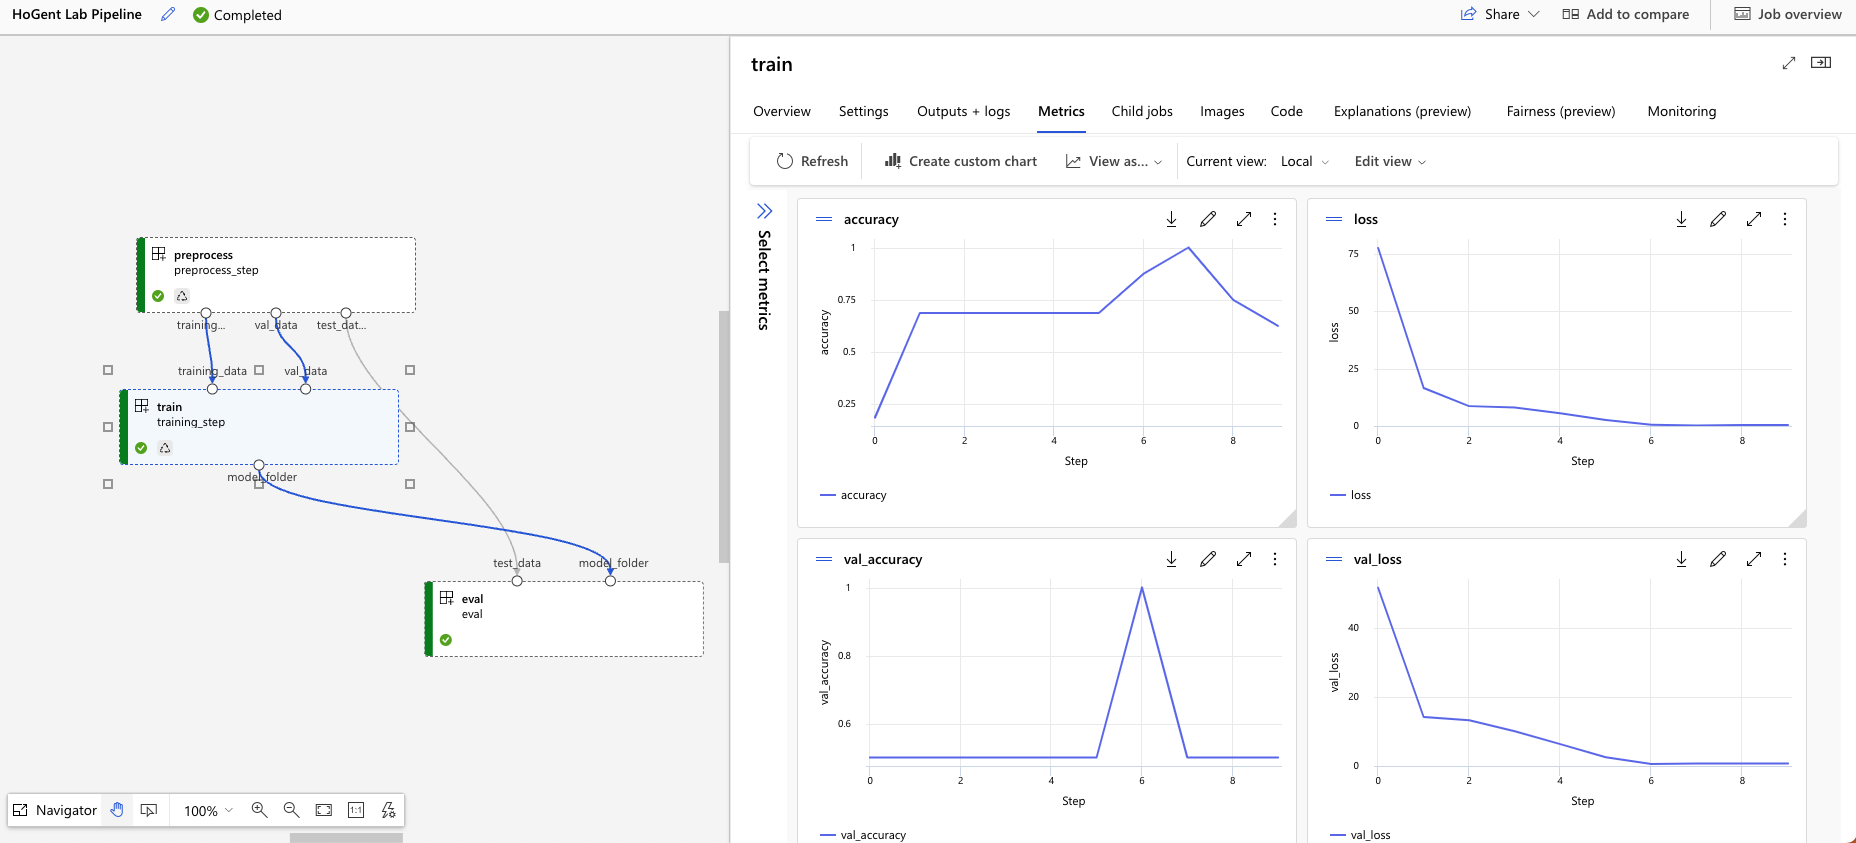
\includegraphics[width=\linewidth]{download.png}
% %     \caption{Flow in Azure, Bron: Machine Learning Operations}
% %     \label{fig:Resultaten in Azure}
% % \end{figure}

% %Figuur \ref{fig:Resultaten in Azure} toont de flow aan hoe de notebook van Machine Learning Operations eruit ziet in een Azure omgeving, hier kan duidelijk gezien worden dat er een flow is van 3 taken.
% Dit werd eerder toegewezen in het scenario, maar hier zie je de 3 taken: preprocessing, train en eval.

% In dit deel van het PoC gaan we het resultaat van labo 3 nabootsen met Prefect.
% Om hier aan te beginnen moeten we eerst het orginele notebook omzetten naar Prefect taken en flows. Er zal gefocust worden op de 3 taken preprocessing, train en eval.

% De preprocessing van het notebook ziet er als volgt uit: 
% \begin{minted}{python}
%     import argparse
%     import glob
%     import os
%     import shutil

%     import cv2
%     import requests

%     IMAGE_SIZE = (150, 150)

%     def _download_from_list(list, type):
%         for i, img_url in enumerate(list):
%             response = requests.get(img_url)
%             response.raise_for_status()

%             ml_split = "train"
%             if i == 9:
%                 ml_split = "test"
%             elif i == 8:
%                 ml_split = "val"

%             with open(f"dataset/{ml_split}/{type}s/{type}{i}.jpeg", "wb") as file:
%                 file.write(response.content)


%     def _get_dataset():
%         for path in [
%             "dataset/train/apples",
%             "dataset/val/apples",
%             "dataset/test/apples",
%             "dataset/train/oranges",
%             "dataset/val/oranges",
%             "dataset/test/oranges",
%         ]:
%             os.makedirs(path)

%         _download_from_list(
%             [
%                 "https://images.unsplash.com/photo-1570913149827-d2ac84ab3f9a?ixlib=rb-4.0.3&ixid=M3wxMjA3fDB8MHxleHBsb3JlLWZlZWR8MXx8fGVufDB8fHx8fA%3D%3D&w=1000&q=80",
%                 "https://thumbs.dreamstime.com/b/red-apple-isolated-clipping-path-19130134.jpg",
%                 "https://images.unsplash.com/photo-1610397962076-02407a169a5b?ixlib=rb-4.0.3&ixid=M3wxMjA3fDB8MHxleHBsb3JlLWZlZWR8Mnx8fGVufDB8fHx8fA%3D%3D&w=1000&q=80",
%                 "https://images.unsplash.com/photo-1568702846914-96b305d2aaeb?ixlib=rb-4.0.3&ixid=M3wxMjA3fDB8MHxwaG90by1wYWdlfHx8fGVufDB8fHx8fA%3D%3D&auto=format&fit=crop&w=2940&q=80",
%                 "https://images.unsplash.com/photo-1576179635662-9d1983e97e1e?ixlib=rb-4.0.3&ixid=M3wxMjA3fDB8MHxwaG90by1wYWdlfHx8fGVufDB8fHx8fA%3D%3D&auto=format&fit=crop&w=2787&q=80",
%                 "https://domf5oio6qrcr.cloudfront.net/medialibrary/11525/0a5ae820-7051-4495-bcca-61bf02897472.jpg",
%                 "https://img.freepik.com/free-photo/two-red-apples-isolated-white_114579-73124.jpg",
%                 "https://t3.ftcdn.net/jpg/01/09/81/46/360_F_109814626_y5dGATGj8h3pMz9tq1HNRfiuXR12uFCj.jpg",
%                 "https://i.pinimg.com/originals/e7/4e/78/e74e782a805bf6f2cc8f178a6063f9d7.jpg",
%                 "https://images.unsplash.com/photo-1584306670957-acf935f5033c?ixlib=rb-4.0.3&ixid=M3wxMjA3fDB8MHxleHBsb3JlLWZlZWR8OHx8fGVufDB8fHx8fA%3D%3D&w=1000&q=80",
%             ],
%             "apple",
%         )

%         _download_from_list(
%             [
%                 "https://plus.unsplash.com/premium_photo-1671013032586-3e9a5c49ce3c?ixlib=rb-4.0.3&ixid=M3wxMjA3fDB8MHxwaG90by1wYWdlfHx8fGVufDB8fHx8fA%3D%3D&auto=format&fit=crop&w=2787&q=80",
%                 "https://images.unsplash.com/photo-1547514701-42782101795e?ixlib=rb-4.0.3&ixid=M3wxMjA3fDB8MHxwaG90by1wYWdlfHx8fGVufDB8fHx8fA%3D%3D&auto=format&fit=crop&w=2787&q=80",
%                 "https://images.unsplash.com/photo-1514936477380-5ea603b9a1ca?ixlib=rb-4.0.3&ixid=M3wxMjA3fDB8MHxwaG90by1wYWdlfHx8fGVufDB8fHx8fA%3D%3D&auto=format&fit=crop&w=2835&q=80",
%                 "https://img.freepik.com/free-photo/orange-white-white_144627-16571.jpg?w=2000",
%                 "https://encrypted-tbn0.gstatic.com/images?q=tbn:ANd9GcRWbb0dC-vAS3Mqx6l_F6uDkUSWFtjHJ8v-MA&usqp=CAU",
%                 "https://static3.depositphotos.com/1000955/120/i/450/depositphotos_1207359-stock-photo-orange.jpg",
%                 "https://publish.purewow.net/wp-content/uploads/sites/2/2021/02/types-of-oranges-navel-oranges.jpg?fit=680%2C489",
%                 "https://encrypted-tbn0.gstatic.com/images?q=tbn:ANd9GcQnS7lPkp0iYsdVraHtEdmNMQ4g7CFNXGZIuFPyNDZamQG29q6K2mLKo1MbSeYfn8NdWoM&usqp=CAU",
%                 "https://encrypted-tbn0.gstatic.com/images?q=tbn:ANd9GcSgA7xpOViT-HeWGzj7f3-rWgX9Fu-dabTj4g&usqp=CAU",
%                 "https://thumbs.dreamstime.com/b/orange-fruit-green-leaves-isolated-white-background-clipping-path-full-depth-field-fresh-177726692.jpg",
%             ],
%             "orange",
%         )


%     def component(training_data, val_data, test_data):
%         _get_dataset()

%         for img_path in glob.glob("dataset/*/*/*.jpeg"):
%             img = cv2.imread(img_path)
%             img = cv2.resize(img, IMAGE_SIZE)
%             img = img.astype("float32") / 255.0
%             cv2.imwrite(img_path, img)

%         shutil.copytree("dataset/train", f"{training_data}/dataset")
%         shutil.copytree("dataset/val", f"{val_data}/dataset")
%         shutil.copytree("dataset/test", f"{test_data}/dataset")


%     if __name__ == "__main__":
%         parser = argparse.ArgumentParser()
%         parser.add_argument("--training_data")
%         parser.add_argument("--val_data")
%         parser.add_argument("--test_data")
%         args = parser.parse_args()

%         component(args.training_data, args.val_data, args.test_data)
% \end{minted}

% De bovenstaande code maakt gebruik van verschillende externe bibliotheken, waaronder argparse, glob, os, shutil, cv2 (OpenCV), en requests, en kan worden verdeeld in volgende stukken:

% \begin{itemize}
%     \item \textbf{Dataset}: Het script gebruikt de requests-module om afbeeldingen van appels en sinaasappels te downloaden van verschillende bronnen op het internet. Deze afbeeldingen worden vervolgens ingedeeld in trainings-, validatie- en testsets, elk met een aparte mapstructuur.
    
%     \item \textbf{preprocessing}: Na het downloaden worden de afbeeldingen verwerkt met behulp van OpenCV (cv2). Elke afbeelding wordt herschaald naar een standaardformaat van 150x150 pixels en genormaliseerd, zodat deze gereed is voor verwerking door een machine learning-model.
    
%     \item \textbf{folder structuur}: Na de verwerking worden de afbeeldingen georganiseerd in de mappen voor de trainings-, validatie- en testsets.
% \end{itemize}

% De volgende code geeft het zelfde resultaat maar dan gebruikmakend van het Prefect framework:

% \begin{minted}{python}
% @task
% def download():
%     for path in [
%         "dataset/train/apples",
%         "dataset/val/apples",
%         "dataset/test/apples",
%         "dataset/train/oranges",
%         "dataset/val/oranges",
%         "dataset/test/oranges",
%     ]:
%         os.makedirs(path, exist_ok=True)


%     def download_from_list(list, type):
%         for i, img_url in enumerate(list):
%             response = requests.get(img_url)
%             response.raise_for_status()

%             ml_split = "train"
%             if i == 9:
%                 ml_split = "test"
%             elif i == 8:
%                 ml_split = "val"

%             with open(f"dataset/{ml_split}/{type}s/{type}{i}.jpeg", "wb") as file:
%                 file.write(response.content)


%     download_from_list(
%         [
%             "https://images.unsplash.com/photo-1570913149827-d2ac84ab3f9a?ixlib=rb-4.0.3&ixid=M3wxMjA3fDB8MHxleHBsb3JlLWZlZWR8MXx8fGVufDB8fHx8fA%3D%3D&w=1000&q=80",
%             "https://thumbs.dreamstime.com/b/red-apple-isolated-clipping-path-19130134.jpg",
%             "https://images.unsplash.com/photo-1610397962076-02407a169a5b?ixlib=rb-4.0.3&ixid=M3wxMjA3fDB8MHxleHBsb3JlLWZlZWR8Mnx8fGVufDB8fHx8fA%3D%3D&w=1000&q=80",
%             "https://images.unsplash.com/photo-1568702846914-96b305d2aaeb?ixlib=rb-4.0.3&ixid=M3wxMjA3fDB8MHxwaG90by1wYWdlfHx8fGVufDB8fHx8fA%3D%3D&auto=format&fit=crop&w=2940&q=80",
%             "https://images.unsplash.com/photo-1576179635662-9d1983e97e1e?ixlib=rb-4.0.3&ixid=M3wxMjA3fDB8MHxwaG90by1wYWdlfHx8fGVufDB8fHx8fA%3D%3D&auto=format&fit=crop&w=2787&q=80",
%             "https://domf5oio6qrcr.cloudfront.net/medialibrary/11525/0a5ae820-7051-4495-bcca-61bf02897472.jpg",
%             "https://img.freepik.com/free-photo/two-red-apples-isolated-white_114579-73124.jpg",
%             "https://t3.ftcdn.net/jpg/01/09/81/46/360_F_109814626_y5dGATGj8h3pMz9tq1HNRfiuXR12uFCj.jpg",
%             "https://i.pinimg.com/originals/e7/4e/78/e74e782a805bf6f2cc8f178a6063f9d7.jpg",
%             "https://images.unsplash.com/photo-1584306670957-acf935f5033c?ixlib=rb-4.0.3&ixid=M3wxMjA3fDB8MHxleHBsb3JlLWZlZWR8OHx8fGVufDB8fHx8fA%3D%3D&w=1000&q=80",
%         ],
%         "apple",
%     )

%     download_from_list(
%         [
%             "https://plus.unsplash.com/premium_photo-1671013032586-3e9a5c49ce3c?ixlib=rb-4.0.3&ixid=M3wxMjA3fDB8MHxwaG90by1wYWdlfHx8fGVufDB8fHx8fA%3D%3D&auto=format&fit=crop&w=2787&q=80",
%             "https://images.unsplash.com/photo-1547514701-42782101795e?ixlib=rb-4.0.3&ixid=M3wxMjA3fDB8MHxwaG90by1wYWdlfHx8fGVufDB8fHx8fA%3D%3D&auto=format&fit=crop&w=2787&q=80",
%             "https://images.unsplash.com/photo-1514936477380-5ea603b9a1ca?ixlib=rb-4.0.3&ixid=M3wxMjA3fDB8MHxwaG90by1wYWdlfHx8fGVufDB8fHx8fA%3D%3D&auto=format&fit=crop&w=2835&q=80",
%             "https://img.freepik.com/free-photo/orange-white-white_144627-16571.jpg?w=2000",
%             "https://encrypted-tbn0.gstatic.com/images?q=tbn:ANd9GcRWbb0dC-vAS3Mqx6l_F6uDkUSWFtjHJ8v-MA&usqp=CAU",
%             "https://static3.depositphotos.com/1000955/120/i/450/depositphotos_1207359-stock-photo-orange.jpg",
%             "https://publish.purewow.net/wp-content/uploads/sites/2/2021/02/types-of-oranges-navel-oranges.jpg?fit=680%2C489",
%             "https://encrypted-tbn0.gstatic.com/images?q=tbn:ANd9GcQnS7lPkp0iYsdVraHtEdmNMQ4g7CFNXGZIuFPyNDZamQG29q6K2mLKo1MbSeYfn8NdWoM&usqp=CAU",
%             "https://encrypted-tbn0.gstatic.com/images?q=tbn:ANd9GcSgA7xpOViT-HeWGzj7f3-rWgX9Fu-dabTj4g&usqp=CAU",
%             "https://www.tastingtable.com/img/gallery/the-science-behind-seedless-oranges/l-intro-1655473463.jpg",
%         ],
%         "orange",
%     )
% \end{minted}

